\chapter{Future Work Plan}
\label{chap:future}

TODO: needs complete revision. in this chapter i discuss how best to approach the aims & objectsives including the research-questions and hypotheses. I am discussing my methods and methodology here.



From the annual review the following things become clear:
- the aim is basically "Explore using Haskell for Agent-Based Simulation with its benefits and drawbacks".
- The 3 major benefits of the approach I claim
	1. code == spec
	2. can rule out serious class of bugs
	3. we can perform reasoning about the simulation in code
	need to be metricated: e.g. this is really only possible in Haskell and not in Java. This needs thorough thinking about which metrics are used, how they can be aquired, how they can be compared,...
- Why ACE and Social Simulation? Did i only pick these fields because they are easily applicable to the problems I want to solve? Which properties do they exhibit which make them interesting for my problem? Just to say that "Sugarscape and bilateral decentralized bartering is interesting and fascinates me" is not enough in a final viva/thesis/paper.
- Reasoning must be very clear. So far I have 2 ideas for formal reasoning in code:
	1. SIR
		-> my emulation of SD using ABS is really an implementation of the SD model and follows it - they are equivalent
		-> my ABS implementation is the same as / equivalent to the SD emulation
			=> thus if i can show that my SD emulation is equlas to the SD model
			=> AND that the ABS implementation is the same as the SD emulation
			=> THEN the ABS implementation is an SD implementation, and we have shown this in code for the first time in ABS

	2. Decentralized Bilateral Bartering
		-> can we reason about the equilibrium prices in an ABS setting? e.g. show formally why equilibrium prices are not reached, under which circumstance they are reached,...
			-> need to combine General Equilibrium Theory
			-> with Bilateral decentralized exchange
			-> with Agent-Based Simulation 
			
- STILL I NEED TO SHOW HOW I CAN MAKE HASKELL RELEVANT IN THE FIELD OF ABS
	-> as far as I know so far no reasoning has been done in the way I intend to do it in the field of ABS. My hypothesis is that it is really only possible in Haskell due to its explicit side-effects, type-system, declarative style,... 
		-> TODO: need to check if this is really unique to haskell
	-> the functional-reactive approach seems to bring a new view to ABS with an embedded language for explicit time-semantics. Together with parallel/sequential updating this allows implementing System-Dynamics and agents which rely on continuous time-semantics e.g. SIR-Agents. Maybe i invented a hybrid between SD and ABS? Also what about time-traveling? The problem is that this is not really clear as i hypothesize that is completely novel approach to ABS - again I need to check this!
		-> TODO: is this really unique to functional reactive? E.g. what about Repast, NetLogo, AnyLogic, other Java-Frameworks? 
	-> maybe i have to admit that its not as unique as thought

In General i need to show that
- Haskells general benefits \& drawbacks over other Languages in the Field of ABS (e.g. Java, NetLogo, Repast) e.g. declarative style, reasoning, explicit about side-effects, performance, difficult to reason about performance, space-leaks difficult. So this focuses on the general comparison between the established technologies of ABS and Haskell but not yet on Haskells suitability in comparison to these other technologies. Here we talk about reasoning, side-effects, performance IN GENERAL TERMS, NOT SPECIFIC TO ABS. We need to distinguish between 
	-> general technicalities e.g. lambda-calculus (denotational formalism) or turing-machine (operational formalism) foundations, declarative style, lazy-evaluation allows to split the producer from the consumer, explicit about side-effects, not possible for in-order updates,...
	-> and in what they result e.g. fewer lines of code, ruling out of bugs, reasoning, lower performance, difficult to reason about space-time 
	
- Haskells suitability to implement ABS in comparison to other languages and technologies in the Field. Here the focus is on general problems in ABS and how they can and are solved using Haskell e.g. send message, changing environment, handling of time, replications, parallelism/concurrency,...

- Why using Haskell in ABS - do the general benefits / drawbacks apply equally well? Are there unique advantages? Can we do things in Haskell which are not possible in other technologies or just very hard? E.g. the hybrid-approach I created with FRP: how unique is it e.g. can other technologies easily implement it as well? Other potential advantages: recursive simulation. Here we DO NOT concentrate on general technicalities but see how they apply when using it for ABS and if they create a unique benefit for Haskell in ABS.

i need to show that different programming languages and paradigms have different power and are differently well suited to specific problems: the ultimate claim i need to show is that haskell is more powerful than java or C++ - the question is if this also makes it superior in applying it to problems: being more powerful, can all problems of java be solved better in haskell as well? this is i believe not the case e.g. gui- or game- programming. the question then is: what is the power of a programming language? can we measure it?

so what i need to show is how well haskell and its power are suited for implementing ABS. does the fact that haskell is much more powerful than existing technologies in ABS lead to the point that it is better suited for ABS? in fact it is power vs. better suited




TODO: rework old introduction
In this chapter we break down the the four main objectives we have identified in Chapter \ref{chap:aimsObj} into small working packages, present mile-stones and holidays, relevant conferences, papers we want to publish (either conference or journal). A Gantt-Chart, reflecting all the details is found at the end of this chapter in Figure \ref{fig:gantt}.

\section{Planned Papers}
TODO: this is real delicate part. how do we split up our objectives and research-questions in to papers? do they all have to be tretated in papers? 
TODO: after having finalized the objectives and research-questions, only THEN split it into papers. A maximum of 4 papers will leave about 6 months for each paper to work on - is this realistic or should we aim for 3 papers?

\subsection{Programming Paradigms in ABS}
This paper will build on the insights of the sketch paper on Programming Paradigms (TODO: be more precise, I already mentioned it)

\subsection{FrABS - Towards pure functional programming in ABS}
This paper will present the pure functional approach to ABS we have taken and outlined in Appendix \ref{app:frABS}. It will describe the combination of FRP \& ABS, the EDSL built on top and discusses its benefits using the SIR model which is implemented both as a ABS and a System-Dynamcis solution. We will show that both implementations are qualitatively the same by reasoning about the simulation. Also implement an STM version of FrABS and look into it.

\subsection{Will it Equilibrate? Reasoning in pure functional ABS}
In this paper we will discuss the verification method we have developed using our FrABS implementation and QuickCheck. We describe the decentralized bilateral bartering process of the Sugarscape model and verify it.
-> purely reasoning about the bilateral trading in sugarscape.
	-> explain bilateral decentralized bartering
	-> general equilibrium theory
	-> give reason in code for the failure of reaching equilibrium

\subsection{Time-travel in ABS}
	-> this paper looks into the specifics of the hybrid approach of FrABS: how time can be used. It asks if time can be turned back e.g. that time-travel may become possible. This facility would pose interesting new mechanisms for investigating the dynamics of Agent-Based Simulations: halting time, fast-forward and fast-backward. The backward-going is a novelty. Could we inject new random-seeds during execution? 
	
\section{Years Overview}

\subsection{1st Year}
In the first year, all is about orientation, experimenting and finding out what the PhD is \textit{really} going to be about. The aim is to have a good working prototype of the library with a few good examples - including SugarScape and Agent\_Zero ready. 

\subsection{2nd Year}
In the second year, the focus will be on \textit{verification}. Using the FrABS library and QuickCheck we will research how far we can go into formalizing model-specifications and how well we can do verification. 

\subsection{3rd Year}
Tocus on cleaning up the research and writing the final thesis. The plan is to start the writing of the final thesis around April 2019 with a 5-months writing-window and to submit on-time at end of September 2019.

\section{Conferences}
\begin{itemize}
	\item \textbf{Multi-Agent Systems AAMS} - General Multi-Agent Systems and Agent-Based Modelling \& Simulation, Deadline in November
	\item \textbf{Social Simulation Conference SSC} - New Methods and models in simulation, Deadline in March
	\item \textbf{Symposium on Trends in Functional Programming} - Functional programming stuff, Deadline in May
\end{itemize}

\section{Mile-Stones}
\begin{itemize}
	\item 2017 31st March - finished and submit Paper 
	\item 2017 18th June - Finished writing 1st year report 
	\item 2017 21st July - 1st Annual Review
	\item 2017 October - 2nd year starts
	\item 2018 May - Submit Paper on FrABS
	\item 2018 October - 3rd year starts
	\item 2019 February - Submit Paper on Verification
	\item 2019 April - Begin of thesis-writing
	\item 2019 September - Submit Thesis
	\item 2019 30th September - official end of PhD
	\item 2020 30th September - end of pending-period
\end{itemize}

\label{app:gantt}
\begin{landscape}
	\begin{figure}
		\label{fig:gantt}
  		\caption{Gantt-Chart for remaining PhD}
  		\centering
  		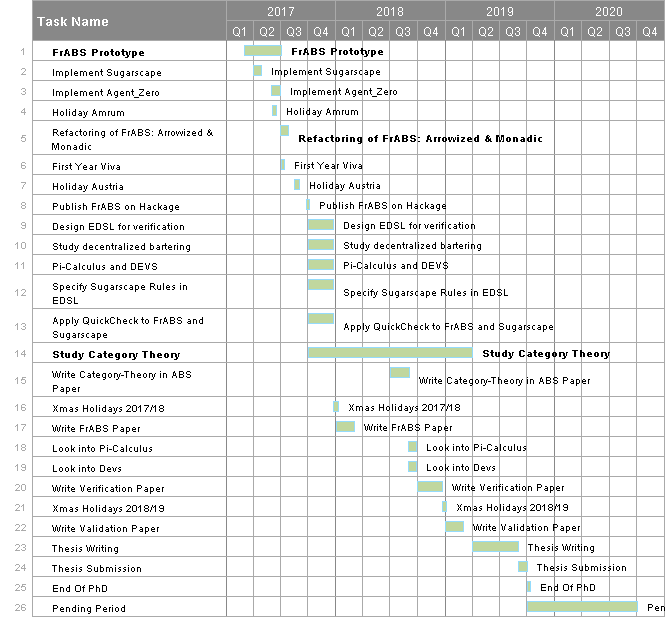
\includegraphics[width=1.2\textwidth]{./charts/gantt.png}
	\end{figure}
\end{landscape}